\chapter{Background and Literature Review} \label{chap:sota}

\minitoc \mtcskip \noindent

This section aims the analysis and reflection about some works that has as final goal, similarly to ours, the development of a framework with the purpose of exploring social media data to extract meaningful domain-specific information. Nonetheless, studying works from other authors may help or even find already proposed solutions in order to solve the aforementioned problems.

Hence, this section will contemplate a brief contextualization about how can an intelligent system contribute to the improvement of a \textit{smart city} or transportation services. Moreover, technologies and methods that allow extraction of information from a text document or, in this particular case, from tweets will be described. Finally, an exploration through already existent frameworks regarding the information extraction from social media content as well as the identification of its application domain.

\section{Smart Cities}\label{sec:smart_cities}

\textit{Smart City} is a concept appeared thanks to the continuous growth of a city's population which contributed to an aggressive level of urban and technological developments~\cite{kn:Cecilia2016}. In the last few years, several definitions for its meaning have emerged but its main idealization is not yet fully known~\cite{kn:Komninos2009}. M. Angelidou~\cite{kn:Angelidou2015} defined Smart City as

\emph{Conceptual urban development model on the basis of the utilization of human, collective, and technological capital for the development of urban agglomerations.}

enhancing \textit{knowledge} and \textit{innovation economy} as the primary factors that support the development of a city. The author identifies four distinct forces that shape the concept of a \textit{smart city}, being two of them :

\begin{enumerate}
	\item \textit{Technology Push}: The need of new products and solutions are introduced into the market due to a fast advance in science and technology.
	\item \textit{Demand Pull}: Current problems are solved originating new possibilities to respond society demands such as the continuous growth of the population.
	\item \textit{Urban Future}: Represents the final goal of a city constituting for that reason an important role in the whole transformation process.
	\item \textit{Knowledge and Innovation Economy}: The creation of new products using the most recent technologies is associated to solution for the efficiency and sustainability of a city.
\end{enumerate}

The first two forces previous mentioned are directly dependent of the other ones as it is showed in Figure~\ref{fig:four_forces}. However, the absence of desire to reach a better future having into consideration the city's economy and resources can result in the break of its dynamics and healthy, affecting services of a city due to the population discontentment.

\begin{figure}
	\centering
	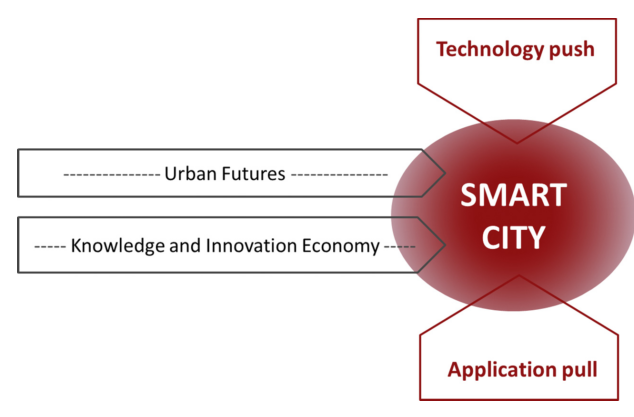
\includegraphics[width=0.6\textwidth]{figures/four_forces.png}
	\caption{\textit{Smart City} conjecture of four forces. Source:~\cite{kn:Angelidou2015}}
	\label{fig:four_forces}
\end{figure}

The development environment of a city tagged as \textit{smart} is another key factor to reach the success. N. Komninos~\cite{kn:Komninos2009} associates collective sources of innovation to the improvement of life quality in cities. The globalization of innovation networks is responsible for the emergency of another types of environments and infrastructures, as so \emph{global innovation clusters and i-hubs, intelligent agglomerations, intelligent technology districts and intelligent clusters, living labs} allowing the testing of products or services by the ordinary citizens in order to identify problems or even analyse their behaviour  and reactions regarding what have experimented~\cite{kn:Komninos2009}. Hence, it is possible to affirm that the development of a city has its starting point in the community but also depends on the quality of Information and Communications Technologies (ICT)~\cite{hollands2008will}, an essential requirement in the city's evolution process.

Last but not least, a \textit{smart city} may focus its efforts in several sectors, such as the environment, culture and recreation, education, social and economic aspects, demography, and travel and transportation~\cite{caragliu2011smart} in order to have equally advances in all of it.

\section{Intelligent Transportation Systems}\label{sec:intelligent_transportation_systems}

The transportation system is inherently connected to the progress of a city because people uses on a daily-basis transportation modes, i.e. bus, private cars, metropolitan, and others, in order to go to their jobs and make their own life and through that they contribute to the economic progress of it. Although this connection, such system is also influenced by the problem of population growth being relevant and necessary the finding of solutions to minimize or even erase it~\cite{kn:Caragliu2015}. Hence, \emph{a smart city should be focused on its actions to become smart}, coming up the concept of innovation~\cite{kn:Cecilia2016}.

To understand what are \textit{Intelligent Transportation Systems} (ITS), it is crucial introduce the meaning of Smart Mobility (SM). SM is a combination of comprehensive and smarter traffic service with smart technology, enabling several intelligent traffic systems which provide control in the signals regarding the traffic volume, information about smooth traffic flows, times of bus, train, subway and flight arrivals, their routes or even the knowledge of what citizens thought about the city's services\cite{kn:Chun2015}. The majority of \textit{Intelligent Transportation Systems} are expressed through smart applications where transportation and traffic management has became more efficient and practicable, allowing the users to access important information about the transportation systems in order to make correct decisions about what they want to use in their cities \cite{kn:Caragliu2015}. ICT-based infrastructures are the main support for \textit{smart cities} and due to tha, they also serve as support to ITS, since the information provide by such infrastructures allows the piloting of activities such as traffic operations, as well as its  management over a long period of time \cite{kn:Cecilia2016}.

Nowadays, cities are exploring some initiatives of sensing to support the development of technological projects. Areas such as utilities management (where, for example, is monitored the consumption level of power, water and gas), traffic management (using vibration sensors to measure the traffic flows on bridges, or even the full capacity of a parking lot), environment awareness (using video cameras to monitor the population behaviour and sensors to measure the level of air pollution) make use of physical sensors, i.e. some devices that can capture information to study and improve the quality of life in a daily basis \cite{kn:Doran2015}. R. Szabo et al.~\cite{kn:Szabo2013} and D. Doran et al.~\cite{kn:Doran2015} reported the highly economic cost to this kind of sensing, since it is require maintenance and replacement of this devices, as well as a tracking infrastructure to store and process the collected information. Hence, a new form of sensing has emerged - Crowd Sensing - offering to cities several ways to improve their services by exploring the participation of the citizens through social networks where there is a publicly sharing of  opinions and thoughts regarding some problems around the city where they live are passing in~\cite{kn:Roitman2012}. This type of sensing consists in \textit{human-generated} data provided by the population through the usage of mobile devices and social networks web-based platforms. Such data can be further used to extract some analytics regarding specific services in a city, namely the urban transportation system \cite{kn:Roitman2012}. Based on all this, social media can be seen as a good source of data to extract valuable information aiming the direct use of it into the smartness evolution process of a city \cite{kn:Szabo2013}. 


\section{To be Defined}

Several works have already been developed and presented taking into account these two large areas, Transportation Services and Smart Cities, using social media as source of information.
G. Anastasi et al. \cite{kn:Anastasi2013} proposed a framework which objective was the promotion of flexible transportation systems usage, i.e. encouraging people to share transport or to opt for the use of bicycles in order to minimize infrastructural and environmental problems. Their tool takes advantages of the crowd sensing techniques by exploring social media streams to predict accidents or traffic congestion and alert the users of their service about this type of events.
W. Liu et al. \cite{kn:Liu2012} have made a study in three different transportation modes (private cars, public transportations and bicyclists) using theirs channels on Twitter to estimate a percentage of the majority gender that uses this services in the city of Toronto. They have extract all the channel's tweets appealing only to the \textit{non-protected} followers and applied an already developed classification model to label each tweet with its creator gender: male or female.

T. Ludwig et al. \cite{kn:Ludwig2015} proposed a tool capable of collect and display social media streams in order to help the integration and coordination of volunteers in actions performed by emergency services to prevent engagement in dangerous areas. Their tool present to the end-users map visualization of a city where they could identify public calls of the emergency services to accept or deny them.

In conclusion to everything that has been analyzed in this sub-section, it's possible to verify that the cities are increasingly opting for technological opportunities that involve crowd sensing, once this type of exploration brings a considerable reduction of costs and the information that is collected may contribute to the extraction of value from data generated by the population itself.

